\documentclass[11pt]{article}
\usepackage[margin=1in]{geometry}
\usepackage[T1]{fontenc}
\usepackage[utf8]{inputenc}
\usepackage{lmodern}
\usepackage{setspace}
\usepackage{hyperref}
\usepackage{xcolor}
\usepackage{listings}
\usepackage{longtable}
\usepackage{array}
\usepackage{titlesec}
\usepackage{fancyhdr}
\usepackage{graphicx}

\hypersetup{
  colorlinks=true,
  linkcolor=blue,
  urlcolor=blue,
  citecolor=blue
}

\lstdefinestyle{mystyle}{
  basicstyle=\ttfamily\small,
  breaklines=true,
  columns=fullflexible,
  keepspaces=true,
  frame=single,
  showstringspaces=false,
  keywordstyle=\color{blue},
  commentstyle=\color{teal},
  stringstyle=\color{purple}
}
\lstset{style=mystyle}

\titleformat{\section}{\large\bfseries}{\thesection.}{0.5em}{}
\titleformat{\subsection}{\normalsize\bfseries}{\thesubsection}{0.5em}{}

\pagestyle{fancy}
\fancyhf{}
\rhead{INFSCI 1540 Final Report}
\lhead{Climate Data Warehouse Project}
\cfoot{\thepage}

\title{INFSCI 1540 - Data Engineering\\Climate Data Warehouse Project\\\large Final Report}
\author{Boyi Sun \and Murphy Zhao}
\date{\today}

\begin{document}
\maketitle
\onehalfspacing

\section{Project Overview}
This project builds a climate data warehouse based on NOAA Climate Data Online data. The whole project can be founded in It uses Docker, Kafka, ksqlDB, MySQL, and Python to support data ingestion, cleaning, transformation, and storage. The system organizes climate normal data in a STAR schema with fact and dimension tables, and also creates pre-aggregated monthly summary tables for efficient analysis. By integrating multiple weather stations into the pipeline, the project supports comparative climate analysis across locations and time periods. All project materials are available in the project GitHub repository: \href{https://github.com/Boyiiiisun/INFSCI1540-Project-Climate}{https://github.com/Boyiiiisun/INFSCI1540-Project-Climate}.


\section{Data Description}
This project maintains climate normal data derived from the NOAA Climate Data Online source. The data source is available at \href{https://www.ncei.noaa.gov/cdo-web/}{https://www.ncei.noaa.gov/cdo-web/}, and the implementation in the current repository is based on the \texttt{NORMAL\_DLY} sample file, which stores daily normal measurements for multiple weather stations. The data pipeline currently preserves four stations in the repository sample: \textit{PETERSBURG 2 N ND US}, \textit{PITTSBURGH INTL AP PA US}, \textit{SEATTLE URBAN SITE WA US}, and \textit{SAN FRANCISCO OCEANSD CA US}. Each record is associated with one station and one calendar date.

The source file contains the following attributes: station identifier, station name, elevation, latitude, longitude, date, daily minimum temperature normal, daily maximum temperature normal, and month-to-date precipitation normal. The system preserves station metadata together with daily climate observations so that the data warehouse can support time-based analysis, station-based comparison, and pre-aggregated monthly summaries.

The grain of the main fact data in the warehouse is one climate normal observation for one station on one date. This design allows the system to support both daily-level analysis and month-level summaries derived from the daily observations.

\section{Docker Containers Used in the System and Corresponding \texttt{docker-compose.yml}}
The system is deployed through Docker Compose. The repository uses containerized infrastructure to isolate operational data storage, warehouse storage, streaming middleware, and query interfaces. The main containers are summarized below.

\subsection{Container Roles}
\begin{itemize}
    \item \textbf{web-server}: a lightweight Apache/PHP container used as a simple web server.
    \item \textbf{mysql-odb-server}: the MySQL instance that stores the operational database (ODB) raw table.
    \item \textbf{mysql-dw-server}: the MySQL instance that stores the dimensional warehouse tables and summary tables.
    \item \textbf{phpmyadmin-odb}: a browser-based administration interface for the ODB MySQL instance.
    \item \textbf{phpmyadmin-dw}: a browser-based administration interface for the DW MySQL instance.
    \item \textbf{zookeeper}: the coordination service required by Kafka in this environment.
    \item \textbf{broker}: the Kafka broker that receives raw JSON messages from the producer and exposes them to downstream consumers and ksqlDB.
    \item \textbf{ksqldb-server}: the ksqlDB server used for stream definition, cleaning, transformation, and monthly aggregation.
    \item \textbf{ksqldb-cli}: the command-line client used to execute ksql statements interactively.
\end{itemize}

This container layout separates storage and streaming concerns. The ODB is used as a staging layer for cleaned operational records, while the DW stores the star schema and summary tables. Kafka and ksqlDB provide the streaming and transformation layer between ingestion and warehouse analytics.

After running \texttt{docker-compose up -d} in the terminal, the Docker environment starts all required services for the project. The screenshot below shows the running containers, confirming that the ODB, DW, Kafka, ksqlDB, phpMyAdmin, and web-server components were successfully launched before the data preparation and warehouse loading steps.

\begin{center}
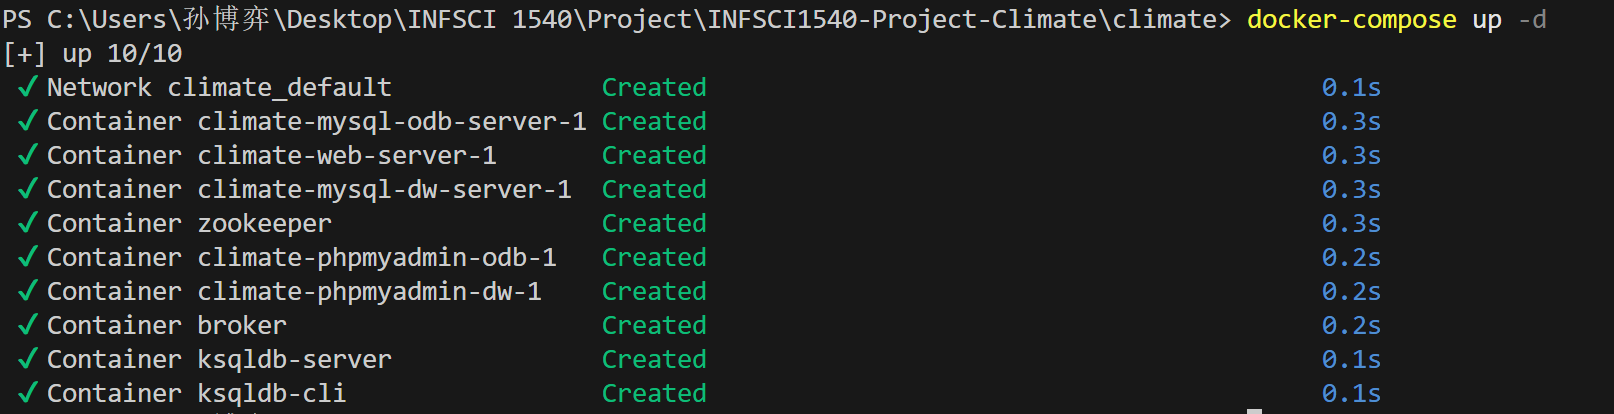
\includegraphics[width=0.95\textwidth]{container.png}
\end{center}

\subsection{Docker Compose File}
\begin{lstlisting}[language={}]
#version: '2'

services:
  web-server:
    image: php:7.4.3-apache
    volumes:
      - "./html/:/var/www/html/"
    ports:
      - "8080:80"

  mysql-odb-server:
    image: mysql:8.0.23
    platform: linux/amd64
    environment:
      MYSQL_ROOT_PASSWORD: secret
    volumes:
      - mysql-odb-data:/var/lib/mysql
    ports:
      - "13306:3306"

  mysql-dw-server:
    image: mysql:8.0.23
    platform: linux/amd64
    environment:
      MYSQL_ROOT_PASSWORD: secret
    volumes:
      - mysql-dw-data:/var/lib/mysql
    ports:
      - "23306:3306"

  phpmyadmin-odb:
    image: phpmyadmin/phpmyadmin:5.0.1
    platform: linux/amd64
    environment:
      PMA_HOST: mysql-odb-server
      PMA_USER: root
      PMA_PASSWORD: secret
    ports:
      - "15000:80"
    depends_on:
      - mysql-odb-server

  phpmyadmin-dw:
    image: phpmyadmin/phpmyadmin:5.0.1
    platform: linux/amd64
    environment:
      PMA_HOST: mysql-dw-server
      PMA_USER: root
      PMA_PASSWORD: secret
    ports:
      - "25000:80"
    depends_on:
      - mysql-dw-server

  zookeeper:
    image: confluentinc/cp-zookeeper:7.9.4
    platform: linux/amd64
    hostname: zookeeper
    container_name: zookeeper
    ports:
      - "2181:2181"
    environment:
      ZOOKEEPER_CLIENT_PORT: 2181
      ZOOKEEPER_TICK_TIME: 2000

  broker:
    image: confluentinc/cp-enterprise-kafka:7.9.4
    platform: linux/amd64
    hostname: broker
    container_name: broker
    depends_on:
      - zookeeper
    ports:
      - "29092:29092"
    environment:
      KAFKA_BROKER_ID: 1
      KAFKA_ZOOKEEPER_CONNECT: "zookeeper:2181"
      KAFKA_LISTENER_SECURITY_PROTOCOL_MAP: PLAINTEXT:PLAINTEXT,PLAINTEXT_HOST:PLAINTEXT
      KAFKA_ADVERTISED_LISTENERS: PLAINTEXT://broker:9092,PLAINTEXT_HOST://localhost:29092
      KAFKA_OFFSETS_TOPIC_REPLICATION_FACTOR: 1
      KAFKA_GROUP_INITIAL_REBALANCE_DELAY_MS: 0
      KAFKA_TRANSACTION_STATE_LOG_MIN_ISR: 1
      KAFKA_TRANSACTION_STATE_LOG_REPLICATION_FACTOR: 1
  
  ksqldb-server:
    image: confluentinc/cp-ksqldb-server:7.9.6-1-ubi8
    platform: linux/amd64
    hostname: ksqldb-server
    container_name: ksqldb-server
    depends_on:
      - broker
    ports:
      - "8088:8088"
    environment:
      KSQL_LISTENERS: http://0.0.0.0:8088
      KSQL_BOOTSTRAP_SERVERS: broker:9092
      KSQL_KSQL_LOGGING_PROCESSING_STREAM_AUTO_CREATE: "true"
      KSQL_KSQL_LOGGING_PROCESSING_TOPIC_AUTO_CREATE: "true"
      CONFLUENT_SUPPORT_METRICS_ENABLE: "false"

  ksqldb-cli:
    image: confluentinc/cp-ksqldb-cli:7.9.6-1-ubi8
    platform: linux/amd64
    container_name: ksqldb-cli
    depends_on:
      - broker
      - ksqldb-server
    entrypoint: /bin/sh
    tty: true

volumes:
  mysql-odb-data:
  mysql-dw-data:
\end{lstlisting}

\section{Data Preparation Process, Cleaning, and Transformation}
The data preparation process is implemented as a multi-stage pipeline.

\subsection{Step 1: CSV Ingestion into Kafka}
The script \texttt{dly\_producer.py} reads the source CSV file and publishes one JSON message per record to the Kafka topic \texttt{NORMAL\_DLY\_RAW}. During this step, the script performs basic type conversion. Numerical values such as elevation, latitude, longitude, and the three climate measures are converted from text into numeric Python values before the record is published.

\subsection{Step 2: Loading Raw Operational Data into ODB}
The script \texttt{consumer.py} consumes messages from \texttt{NORMAL\_DLY\_RAW} and writes them into the operational database table \texttt{climate\_normal\_daily\_raw}. In this stage, the process performs the following cleaning operations:
\begin{itemize}
    \item parsing the date field from \texttt{YYYYMMDD} into SQL \texttt{DATE} format,
    \item converting numeric values to decimal types,
    \item skipping malformed messages when required attributes are missing,
    \item using \texttt{ON DUPLICATE KEY UPDATE} to avoid duplicate station-date records.
\end{itemize}

The ODB serves as a structured staging area between raw stream ingestion and dimensional loading.

\subsection{Step 3: ksqlDB Stream Cleaning and Transformation}
The repository includes a ksqlDB layer that transforms the raw Kafka topic into analysis-ready streams. First, the raw JSON topic is registered as the ksql stream \texttt{normal\_dly\_raw}. Then the file \texttt{create\_clean\_stream.sql} derives additional time attributes from the raw date string and casts the climate fields into doubles.

\begin{lstlisting}[language=SQL]
CREATE STREAM normal_dly_clean AS
SELECT
  station_id,
  station_name,
  elevation,
  latitude,
  longitude,
  norm_date,
  CAST(SUBSTRING(norm_date, 1, 4) AS INTEGER) AS year_num,
  CAST(SUBSTRING(norm_date, 5, 2) AS INTEGER) AS month_num,
  SUBSTRING(norm_date, 1, 6) AS norm_month,
  CAST(dly_tmin_normal AS DOUBLE) AS dly_tmin_normal,
  CAST(dly_tmax_normal AS DOUBLE) AS dly_tmax_normal,
  CAST(mtd_prcp_normal AS DOUBLE) AS mtd_prcp_normal
FROM normal_dly_raw
EMIT CHANGES;
\end{lstlisting}

This transformation is important because it introduces month-level and year-level attributes that are later used for summary aggregation.

\subsection{Step 4: Loading the Star Schema}
The script \texttt{load.py} reads the cleaned operational data from ODB and populates the warehouse star schema. The process:
\begin{itemize}
    \item extracts unique stations and upserts them into \texttt{dim\_station},
    \item extracts unique dates and inserts them into \texttt{dim\_date},
    \item maps station identifiers to surrogate keys,
    \item loads the fact table \texttt{fact\_daily\_climate\_normal}.
\end{itemize}

This loading step also uses idempotent insertion logic so the process can be rerun without creating duplicate warehouse records.

\section{STAR Schema Design}
The data warehouse uses a classical star schema with one fact table and two dimension tables.

\subsection{Schema Overview}
\begin{figure}[htbp]
\centering
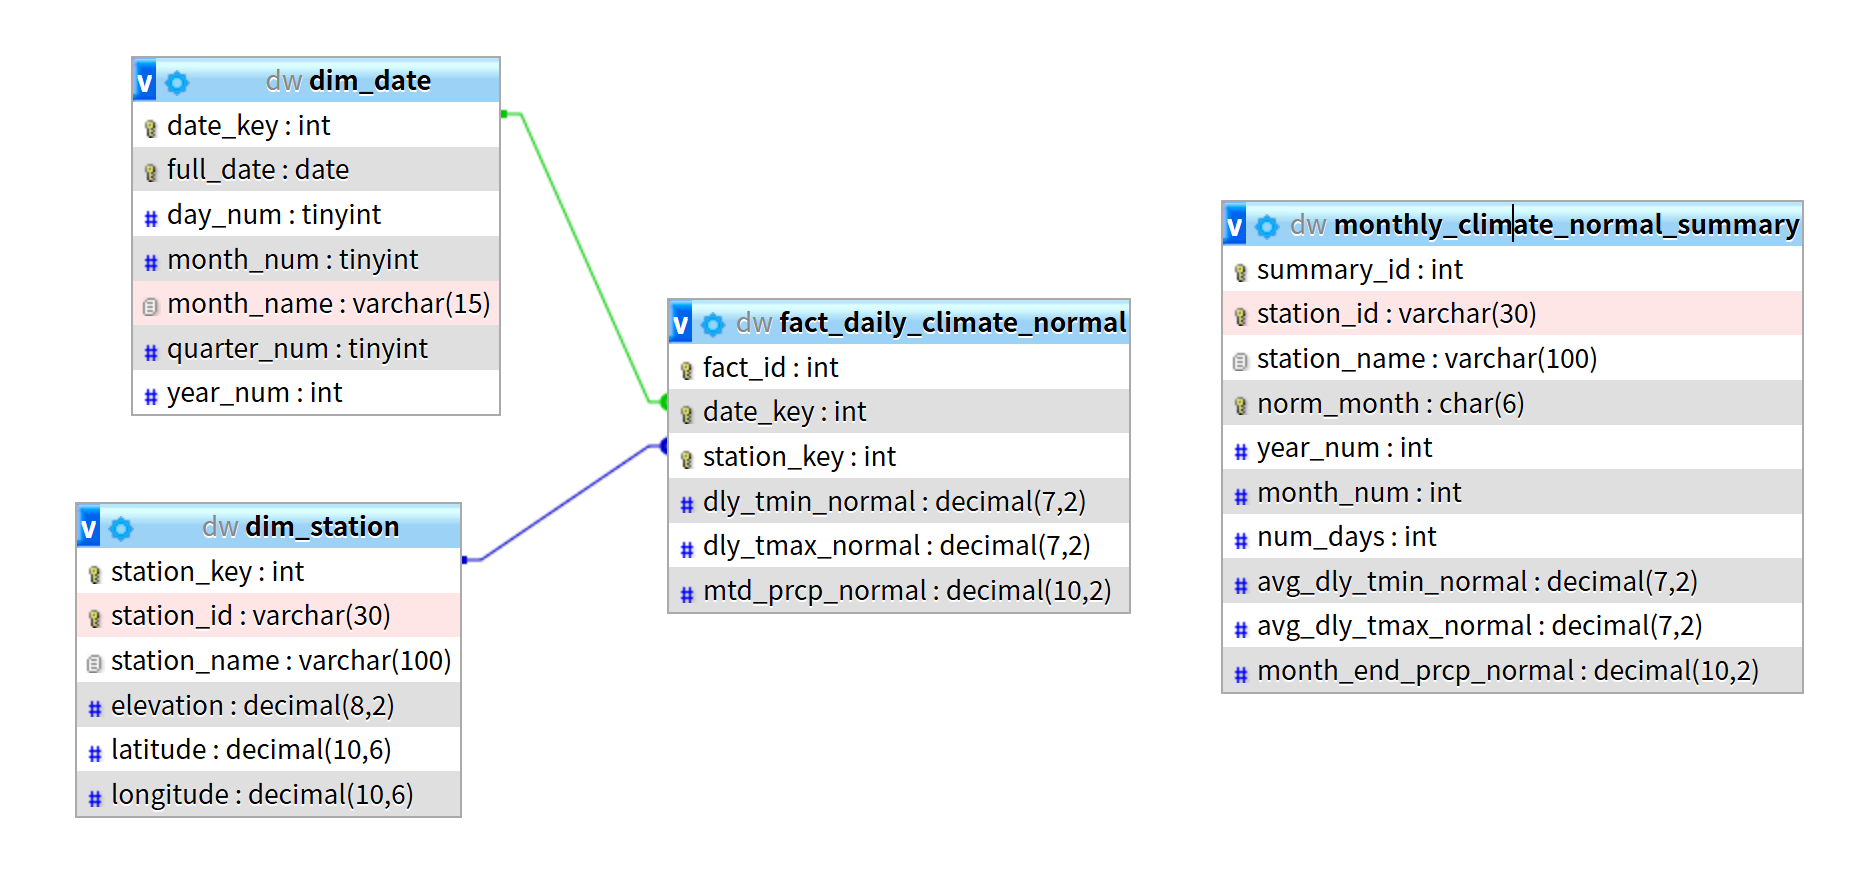
\includegraphics[width=0.9\textwidth]{star_schema.png}
\caption{STAR schema design for the climate data warehouse.}
\end{figure}

The grain of the fact table is one climate normal record for one station on one date.

\subsection{Dimension Table: \texttt{dim\_date}}
\begin{lstlisting}[language=SQL]
CREATE TABLE IF NOT EXISTS dim_date (
    date_key INT NOT NULL PRIMARY KEY,
    full_date DATE NOT NULL,
    day_num TINYINT NOT NULL,
    month_num TINYINT NOT NULL,
    month_name VARCHAR(15) NOT NULL,
    quarter_num TINYINT NOT NULL,
    year_num INT NOT NULL,
    CONSTRAINT uq_dim_date_full_date UNIQUE (full_date)
);
\end{lstlisting}

\subsection{Dimension Table: \texttt{dim\_station}}
\begin{lstlisting}[language=SQL]
CREATE TABLE IF NOT EXISTS dim_station (
    station_key INT NOT NULL AUTO_INCREMENT PRIMARY KEY,
    station_id VARCHAR(30) NOT NULL,
    station_name VARCHAR(100) NOT NULL,
    elevation DECIMAL(8,2) NULL,
    latitude DECIMAL(10,6) NULL,
    longitude DECIMAL(10,6) NULL,
    CONSTRAINT uq_dim_station_station_id UNIQUE (station_id)
);
\end{lstlisting}

\subsection{Fact Table: \texttt{fact\_daily\_climate\_normal}}
\begin{lstlisting}[language=SQL]
CREATE TABLE IF NOT EXISTS fact_daily_climate_normal (
    fact_id INT NOT NULL AUTO_INCREMENT PRIMARY KEY,
    date_key INT NOT NULL,
    station_key INT NOT NULL,
    dly_tmin_normal DECIMAL(7,2) NULL,
    dly_tmax_normal DECIMAL(7,2) NULL,
    mtd_prcp_normal DECIMAL(10,2) NULL,
    CONSTRAINT uq_fact_station_date UNIQUE (station_key, date_key),
    CONSTRAINT fk_fact_daily_normal_date
        FOREIGN KEY (date_key) REFERENCES dim_date(date_key),
    CONSTRAINT fk_fact_daily_normal_station
        FOREIGN KEY (station_key) REFERENCES dim_station(station_key)
);
\end{lstlisting}

\subsection{SQL Statements Used to Populate the STAR Schema}
The warehouse is populated through SQL statements executed by \texttt{load.py}. The main statements are listed below.

\paragraph{Populate \texttt{dim\_station}}
\begin{lstlisting}[language=SQL]
INSERT INTO dim_station (
    station_id, station_name, elevation, latitude, longitude
) VALUES (%s, %s, %s, %s, %s)
ON DUPLICATE KEY UPDATE
    station_name = VALUES(station_name),
    elevation = VALUES(elevation),
    latitude = VALUES(latitude),
    longitude = VALUES(longitude);
\end{lstlisting}

\paragraph{Populate \texttt{dim\_date}}
\begin{lstlisting}[language=SQL]
INSERT IGNORE INTO dim_date (
    date_key, full_date, day_num, month_num, month_name, quarter_num, year_num
) VALUES (%s, %s, %s, %s, %s, %s, %s);
\end{lstlisting}

\paragraph{Populate \texttt{fact\_daily\_climate\_normal}}
\begin{lstlisting}[language=SQL]
INSERT INTO fact_daily_climate_normal (
    date_key, station_key, dly_tmin_normal, dly_tmax_normal, mtd_prcp_normal
) VALUES (%s, %s, %s, %s, %s)
ON DUPLICATE KEY UPDATE
    dly_tmin_normal = VALUES(dly_tmin_normal),
    dly_tmax_normal = VALUES(dly_tmax_normal),
    mtd_prcp_normal = VALUES(mtd_prcp_normal);
\end{lstlisting}

\section{Data Streams}

Following the data warehousing workflow introduced in Lab 7 and the ksqlDB-based stream processing approach in Lab 9, our project uses Kafka and ksqlDB to support real-time ingestion and aggregation of climate data before loading the processed results into the final data warehouse.

\subsection{Overview of the Stream Pipeline}

The data stream pipeline in our project consists of four main stages:

\begin{enumerate}
    \item Climate observation records are read from the prepared source file.
    \item A Python producer sends these records to a Kafka topic.
    \item ksqlDB defines the Kafka topic as a structured stream and performs continuous processing and aggregation.
    \item The aggregated results are loaded into the MySQL data warehouse for multidimensional analysis and OLAP queries.
\end{enumerate}

Compared with the original Lab 7 workflow, our project replaces the intermediate \texttt{odb.transaction} layer with a ksqlDB stream-processing layer. This allows the system to process incoming events directly from Kafka and generate aggregated results in real time.

\subsection{Source Data Stream}

The source data stream contains cleaned climate observation records. Each record represents one weather observation event and includes attributes such as observation date, station identifier, location, measurement type, and observed value.

These records are produced by a Python data producer and sent to a Kafka topic. In our project, this topic serves as the entry point of the streaming pipeline.

\subsection{Kafka Topic and Stream Definition}

After the producer sends the climate records to Kafka, ksqlDB is used to associate a schema with the underlying topic. In this way, raw Kafka messages are interpreted as structured stream records.

The stream definition logically represents the incoming climate events and acts as the streaming equivalent of the original transaction-level input layer. Instead of inserting incoming records into an ODB transaction table first, our project directly defines them as a ksqlDB stream.

\subsection{Continuous Query Processing}

To monitor incoming events, we use a continuous query over the climate event stream. This query continuously outputs new rows as data arrives in the Kafka topic.

This mechanism is useful for validating that the data producer is sending records correctly and that the stream pipeline is functioning as expected. It also demonstrates the real-time nature of the system, since newly produced climate observations immediately become visible in the stream query results.

\subsection{Continuous Aggregation with ksqlDB}

After the climate event stream is created, ksqlDB is used to define a continuous aggregation query. This query groups incoming records by selected attributes and incrementally computes aggregate values as new events arrive.

For our climate data warehouse, this aggregation step can be used to compute summarized measures such as monthly average temperature, monthly maximum temperature, monthly minimum temperature, and monthly total precipitation by station.

The aggregated output is maintained as a ksqlDB table. This table replaces the aggregation logic that was originally implemented in Lab 7 through the \texttt{odb\_producer.py} script and the SQL query over the \texttt{transaction} table.

\subsection{Loading Aggregated Results into the Data Warehouse}

The aggregated results produced by ksqlDB are then loaded into the MySQL data warehouse. These results populate the fact table and support the creation of pre-aggregated summary tables.

The MySQL data warehouse remains the final storage layer of the project. It is used to maintain the STAR schema, support joins with dimension tables, and execute OLAP queries for climate trend analysis.

\subsection{Benefits of the Modified Stream Design}

This modified data stream design provides several advantages:

\begin{itemize}
    \item It simplifies the original Lab 7 pipeline by removing the intermediate ODB transaction storage layer.
    \item It incorporates real-time stream processing using ksqlDB.
    \item It supports continuous aggregation directly on top of Kafka streams.
    \item It better demonstrates the integration of Kafka, ksqlDB, and MySQL in a modern data engineering workflow.
\end{itemize}

Overall, the modified stream architecture allows our project to combine the data warehousing logic of Lab 7 with the stream-processing capabilities of Lab 9, resulting in a more efficient and more scalable climate data pipeline.

\section{Specification of Pre-Aggregated Summary Tables}
The project includes a monthly pre-aggregated summary table in the warehouse and a corresponding aggregated table in ksqlDB.

\subsection{Warehouse Summary Table DDL}
\begin{lstlisting}[language=SQL]
CREATE TABLE IF NOT EXISTS monthly_climate_normal_summary (
    summary_id INT NOT NULL AUTO_INCREMENT PRIMARY KEY,
    station_id VARCHAR(30) NOT NULL,
    station_name VARCHAR(100) NOT NULL,
    norm_month CHAR(6) NOT NULL,
    year_num INT NOT NULL,
    month_num INT NOT NULL,
    num_days INT NULL,
    avg_dly_tmin_normal DECIMAL(7,2) NULL,
    avg_dly_tmax_normal DECIMAL(7,2) NULL,
    month_end_prcp_normal DECIMAL(10,2) NULL,
    CONSTRAINT uq_monthly_normal_station_month UNIQUE (station_id, norm_month)
);
\end{lstlisting}

\subsection{SQL for Creation and Population of Summary Data in ksqlDB}
\begin{lstlisting}[language=SQL]
CREATE TABLE normal_dly_monthly_summary
WITH (
  KEY_FORMAT = 'JSON',
  VALUE_FORMAT = 'JSON'
) AS
SELECT
  station_id,
  AS_VALUE(station_id) AS station_id_v,
  station_name,
  AS_VALUE(station_name) AS station_name_v,
  norm_month,
  AS_VALUE(norm_month) AS norm_month_v,
  year_num,
  AS_VALUE(year_num) AS year_num_v,
  month_num,
  AS_VALUE(month_num) AS month_num_v,
  COUNT(*) AS num_days,
  AVG(dly_tmin_normal) AS avg_dly_tmin_normal,
  AVG(dly_tmax_normal) AS avg_dly_tmax_normal,
  MAX(mtd_prcp_normal) AS month_end_prcp_normal
FROM normal_dly_clean
GROUP BY station_id, station_name, norm_month, year_num, month_num
EMIT CHANGES;
\end{lstlisting}

\subsection{Loading Summary Data into the Warehouse}
The script \texttt{load\_monthly\_summary.py} consumes the summary topic and upserts the aggregated rows into the warehouse summary table using the following SQL pattern.

\begin{lstlisting}[language=SQL]
INSERT INTO monthly_climate_normal_summary (
    station_id,
    station_name,
    norm_month,
    year_num,
    month_num,
    num_days,
    avg_dly_tmin_normal,
    avg_dly_tmax_normal,
    month_end_prcp_normal
) VALUES (%s, %s, %s, %s, %s, %s, %s, %s, %s)
ON DUPLICATE KEY UPDATE
    station_name = VALUES(station_name),
    year_num = VALUES(year_num),
    month_num = VALUES(month_num),
    num_days = VALUES(num_days),
    avg_dly_tmin_normal = VALUES(avg_dly_tmin_normal),
    avg_dly_tmax_normal = VALUES(avg_dly_tmax_normal),
    month_end_prcp_normal = VALUES(month_end_prcp_normal);
\end{lstlisting}

\section{OLAP Data Warehouse Queries}
This section presents five OLAP queries executed against the climate data warehouse. Each query uses the warehouse fact table together with the date and station dimensions to support station comparison, temporal aggregation, and climate pattern analysis.

Before running the OLAP queries, the raw NOAA-style measures are converted into easier-to-read imperial units. In the warehouse, daily minimum and maximum temperature are stored in tenths of degrees Fahrenheit, and month-to-date precipitation is stored in hundredths of inches. To make the analytical results more interpretable, the OLAP workflow first converts temperature values by dividing by 10 and precipitation values by dividing by 100. These converted values are then reused through shared views so that all five queries use the same unit definitions and monthly aggregation logic.

\subsection{Shared Unit Conversion and Monthly Aggregation Views}
\begin{lstlisting}[language=SQL]
USE dw;

-- Convert raw NOAA-style units once:
--   temperature: stored in tenths of degrees Fahrenheit
--   precipitation: stored in hundredths of inches
CREATE OR REPLACE VIEW vw_daily_climate_imperial AS
SELECT
    ds.station_id,
    ds.station_name,
    ds.latitude,
    ds.longitude,
    dd.year_num,
    dd.month_num,
    dd.month_name,
    dd.quarter_num,
    dd.full_date,
    ROUND(f.dly_tmin_normal / 10.0, 2) AS dly_tmin_normal_f,
    ROUND(f.dly_tmax_normal / 10.0, 2) AS dly_tmax_normal_f,
    ROUND(f.mtd_prcp_normal / 100.0, 2) AS mtd_prcp_normal_in
FROM fact_daily_climate_normal f
JOIN dim_date dd
    ON f.date_key = dd.date_key
JOIN dim_station ds
    ON f.station_key = ds.station_key
WHERE
    f.dly_tmin_normal IS NOT NULL
    AND f.dly_tmax_normal IS NOT NULL
    AND f.mtd_prcp_normal IS NOT NULL;

CREATE OR REPLACE VIEW vw_monthly_climate_imperial AS
SELECT
    station_id,
    station_name,
    latitude,
    longitude,
    year_num,
    month_num,
    month_name,
    COUNT(*) AS num_days,
    ROUND(AVG((dly_tmin_normal_f + dly_tmax_normal_f) / 2), 2)
        AS monthly_avg_temperature_f,
    ROUND(MAX(dly_tmax_normal_f), 2) AS monthly_max_temperature_f,
    ROUND(MIN(dly_tmin_normal_f), 2) AS monthly_min_temperature_f,
    ROUND(MAX(mtd_prcp_normal_in), 2) AS monthly_total_precipitation_in
FROM vw_daily_climate_imperial
GROUP BY
    station_id,
    station_name,
    latitude,
    longitude,
    year_num,
    month_num,
    month_name;
\end{lstlisting}

These two views standardize the OLAP input. The first view performs the unit conversion at the daily level, while the second view rolls the converted values into monthly station summaries. All five OLAP queries below read from these views instead of repeating the same conversion and aggregation logic.

\subsection{Query 1: Monthly Climate Summary by Station}
\begin{lstlisting}[language=SQL]
-- OLAP Query 1:
-- Monthly station-level climate summary using converted units.
SELECT
    station_id,
    station_name,
    year_num,
    month_num,
    month_name,
    num_days,
    monthly_avg_temperature_f AS monthly_avg_temperature_normal,
    monthly_max_temperature_f AS monthly_max_temperature_normal,
    monthly_min_temperature_f AS monthly_min_temperature_normal,
    monthly_total_precipitation_in AS monthly_total_precipitation_normal
FROM vw_monthly_climate_imperial
ORDER BY
    station_name,
    year_num,
    month_num;
\end{lstlisting}

\begin{figure}[htbp]
\centering
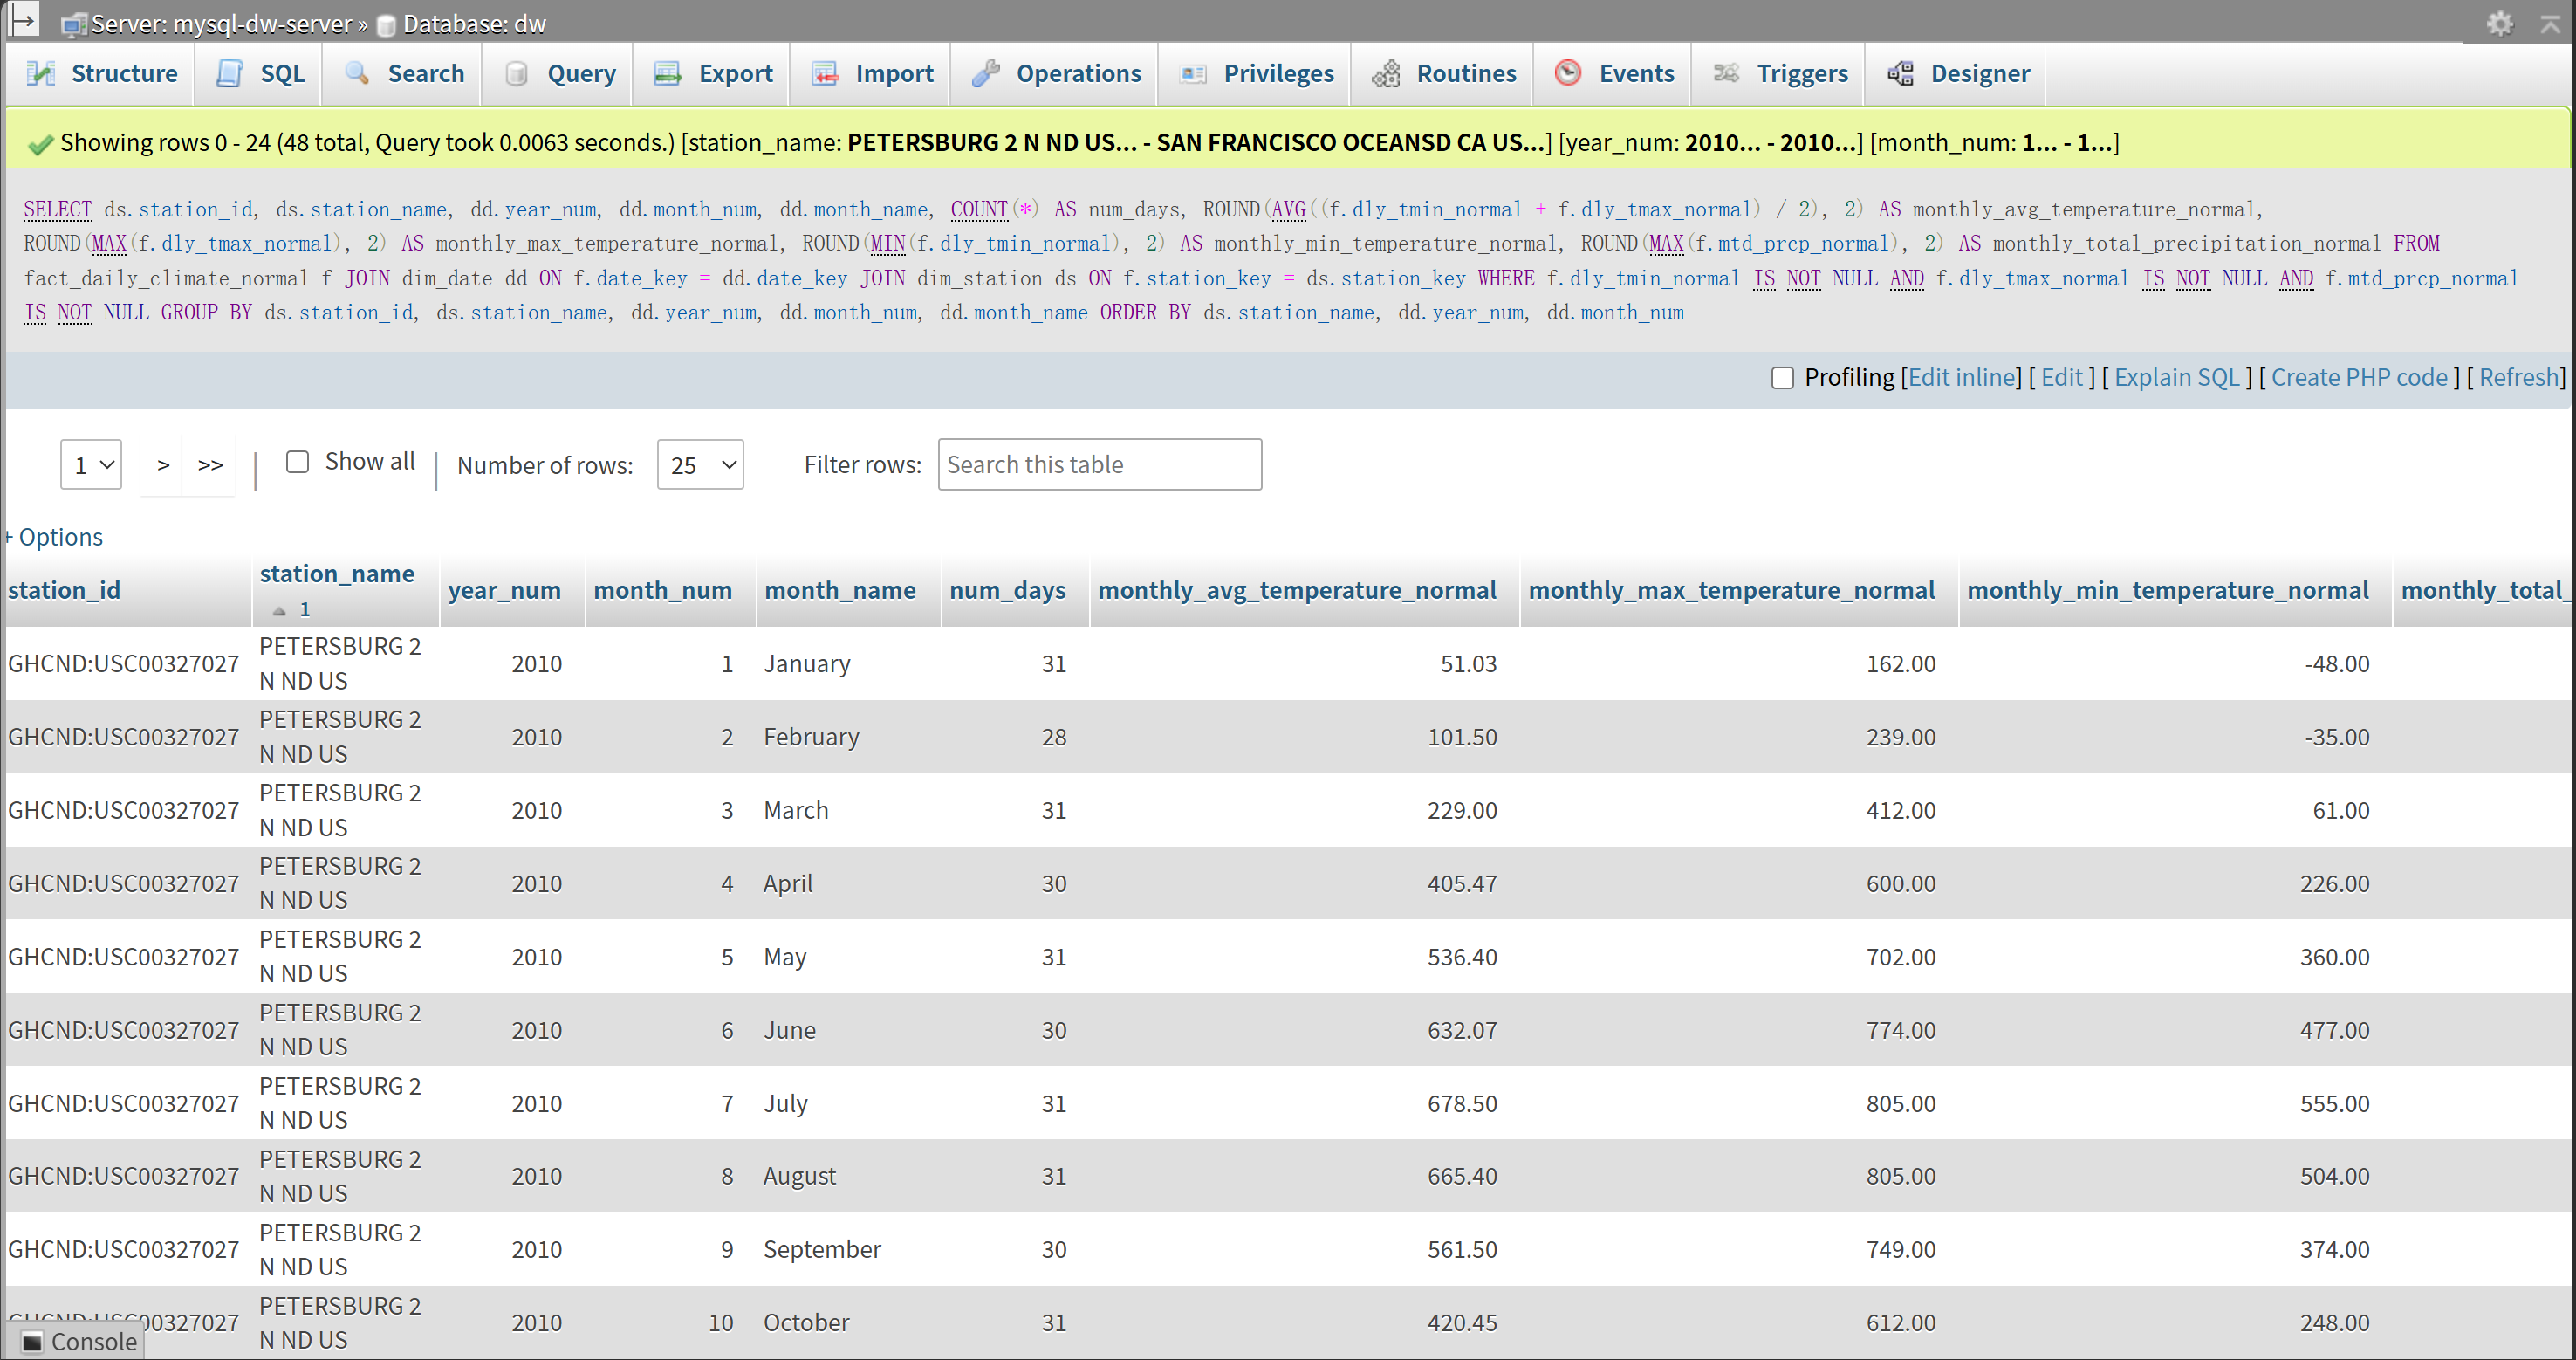
\includegraphics[width=0.95\textwidth]{OLAP_Results/query1.png}
\caption{Result of Query 1: monthly climate summary by station.}
\end{figure}

Query 1 reads directly from the shared monthly view and reports the number of observations, monthly average temperature, monthly maximum temperature, monthly minimum temperature, and monthly precipitation normal for each station. The result is meaningful because it presents monthly summaries in already-converted imperial units, making it easier to compare seasonal climate patterns across all stations.

\subsection{Query 2: Coastal Seattle vs. Inland Petersburg Monthly Comparison}
\begin{lstlisting}[language=SQL]
-- OLAP Query 2:
-- Compare similar-latitude coastal and inland stations:
-- Seattle Urban Site, WA vs Petersburg 2 N, ND.
WITH comparison_months AS (
    SELECT
        year_num,
        month_num,
        month_name,
        MAX(CASE
            WHEN station_id = 'GHCND:USW00024281'
            THEN monthly_avg_temperature_f
        END) AS seattle_avg_temperature,
        MAX(CASE
            WHEN station_id = 'GHCND:USC00327027'
            THEN monthly_avg_temperature_f
        END) AS petersburg_avg_temperature,
        MAX(CASE
            WHEN station_id = 'GHCND:USW00024281'
            THEN monthly_total_precipitation_in
        END) AS seattle_total_precipitation,
        MAX(CASE
            WHEN station_id = 'GHCND:USC00327027'
            THEN monthly_total_precipitation_in
        END) AS petersburg_total_precipitation
    FROM vw_monthly_climate_imperial
    WHERE station_id IN ('GHCND:USW00024281', 'GHCND:USC00327027')
    GROUP BY
        year_num,
        month_num,
        month_name
)
SELECT
    year_num,
    month_num,
    month_name,
    seattle_avg_temperature,
    petersburg_avg_temperature,
    ROUND(
        seattle_avg_temperature - petersburg_avg_temperature,
        2
    ) AS seattle_minus_petersburg_avg_temperature,
    seattle_total_precipitation,
    petersburg_total_precipitation,
    ROUND(
        seattle_total_precipitation - petersburg_total_precipitation,
        2
    ) AS seattle_minus_petersburg_precipitation
FROM comparison_months
ORDER BY
    year_num,
    month_num;
\end{lstlisting}

\begin{figure}[htbp]
\centering
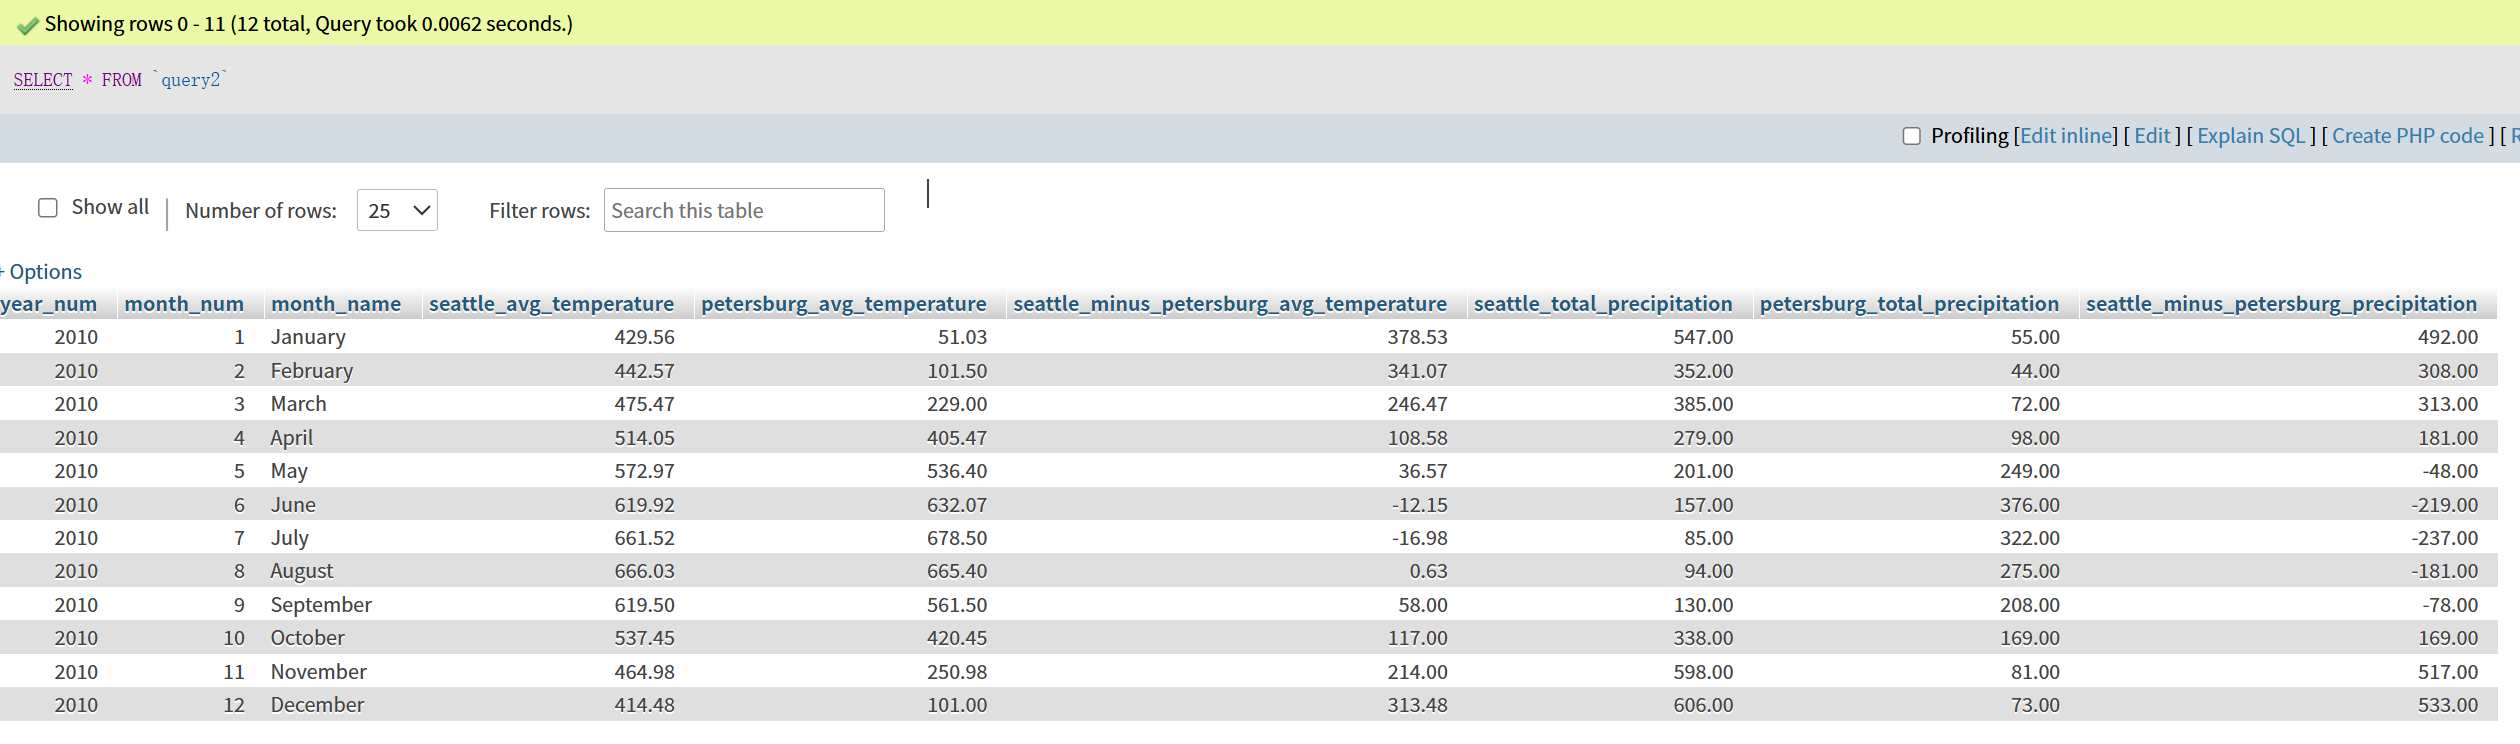
\includegraphics[width=0.95\textwidth]{OLAP_Results/query2.png}
\caption{Result of Query 2: coastal Seattle versus inland Petersburg.}
\end{figure}

Query 2 compares Seattle and Petersburg by pivoting both stations into the same monthly row from the shared monthly view. This layout makes the temperature and precipitation differences directly visible for each month. The result is useful because it highlights the contrast between a coastal station and an inland station, showing how geography can influence both temperature and precipitation normals.

\subsection{Query 3: Seasonal Comparison Between San Francisco and Pittsburgh}
\begin{lstlisting}[language=SQL]
-- OLAP Query 3:
-- Compare San Francisco, CA vs Pittsburgh, PA by season.
WITH seasonal_station AS (
    SELECT
        station_id,
        station_name,
        year_num,
        CASE
            WHEN month_num IN (12, 1, 2) THEN 'Winter'
            WHEN month_num IN (3, 4, 5) THEN 'Spring'
            WHEN month_num IN (6, 7, 8) THEN 'Summer'
            ELSE 'Fall'
        END AS season_name,
        CASE
            WHEN month_num IN (12, 1, 2) THEN 1
            WHEN month_num IN (3, 4, 5) THEN 2
            WHEN month_num IN (6, 7, 8) THEN 3
            ELSE 4
        END AS season_order,
        ROUND(AVG(monthly_avg_temperature_f), 2) AS seasonal_avg_temperature,
        ROUND(MAX(monthly_max_temperature_f), 2) AS seasonal_max_temperature,
        ROUND(MIN(monthly_min_temperature_f), 2) AS seasonal_min_temperature,
        ROUND(SUM(monthly_total_precipitation_in), 2)
            AS seasonal_total_precipitation
    FROM vw_monthly_climate_imperial
    WHERE station_id IN ('GHCND:USC00047767', 'GHCND:USW00094823')
    GROUP BY
        station_id,
        station_name,
        year_num,
        season_name,
        season_order
)
SELECT
    year_num,
    season_name,
    station_name,
    seasonal_avg_temperature,
    seasonal_max_temperature,
    seasonal_min_temperature,
    ROUND(seasonal_max_temperature - seasonal_min_temperature, 2)
        AS seasonal_temperature_range,
    seasonal_total_precipitation
FROM seasonal_station
ORDER BY
    year_num,
    season_order,
    station_name;
\end{lstlisting}

\begin{figure}[htbp]
\centering
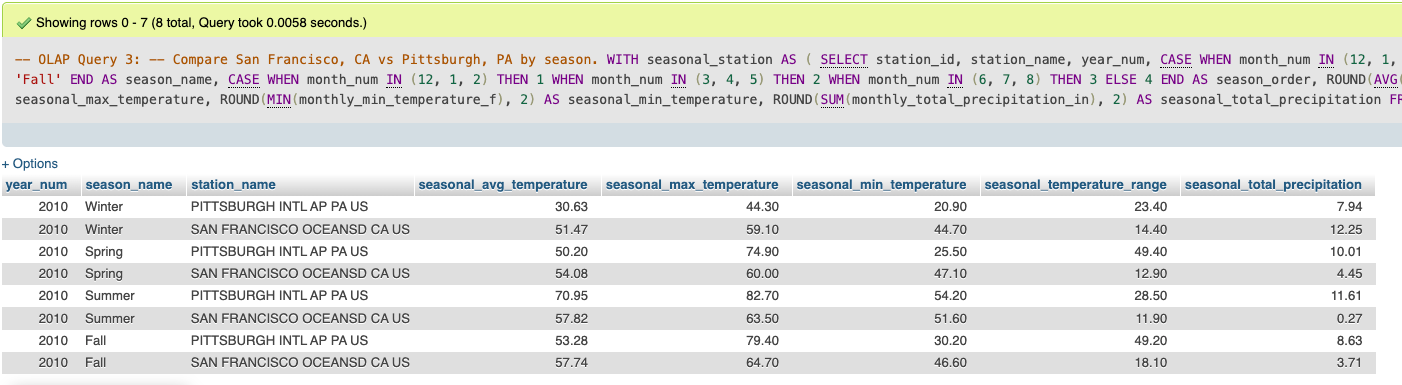
\includegraphics[width=0.95\textwidth]{OLAP_Results/query3.png}
\caption{Result of Query 3: seasonal comparison between San Francisco and Pittsburgh.}
\end{figure}

Query 3 rolls monthly climate values from the shared view into seasonal summaries for San Francisco and Pittsburgh. It reports seasonal average temperature, maximum and minimum normal temperatures, seasonal temperature range, and total precipitation. The result is meaningful because it moves beyond monthly detail and shows broader regional differences, especially the contrast between San Francisco's milder coastal climate and Pittsburgh's stronger seasonal variation.

\subsection{Query 4: Seattle vs. San Francisco Monthly Difference Ranking}
\begin{lstlisting}[language=SQL]
-- OLAP Query 4:
-- Compare Seattle, WA vs San Francisco, CA and rank monthly temperature gaps.
WITH paired_months AS (
    SELECT
        year_num,
        month_num,
        month_name,
        MAX(CASE
            WHEN station_id = 'GHCND:USW00024281'
            THEN latitude
        END) AS seattle_latitude,
        MAX(CASE
            WHEN station_id = 'GHCND:USC00047767'
            THEN latitude
        END) AS san_francisco_latitude,
        MAX(CASE
            WHEN station_id = 'GHCND:USW00024281'
            THEN monthly_avg_temperature_f
        END) AS seattle_avg_temperature,
        MAX(CASE
            WHEN station_id = 'GHCND:USC00047767'
            THEN monthly_avg_temperature_f
        END) AS san_francisco_avg_temperature,
        MAX(CASE
            WHEN station_id = 'GHCND:USW00024281'
            THEN monthly_total_precipitation_in
        END) AS seattle_total_precipitation,
        MAX(CASE
            WHEN station_id = 'GHCND:USC00047767'
            THEN monthly_total_precipitation_in
        END) AS san_francisco_total_precipitation
    FROM vw_monthly_climate_imperial
    WHERE station_id IN ('GHCND:USW00024281', 'GHCND:USC00047767')
    GROUP BY
        year_num,
        month_num,
        month_name
)
SELECT
    year_num,
    month_num,
    month_name,
    seattle_latitude,
    san_francisco_latitude,
    seattle_avg_temperature,
    san_francisco_avg_temperature,
    ROUND(
        san_francisco_avg_temperature - seattle_avg_temperature,
        2
    ) AS san_francisco_minus_seattle_temperature,
    seattle_total_precipitation,
    san_francisco_total_precipitation,
    ROUND(
        san_francisco_total_precipitation - seattle_total_precipitation,
        2
    ) AS san_francisco_minus_seattle_precipitation,
    RANK() OVER (
        ORDER BY ABS(
            san_francisco_avg_temperature - seattle_avg_temperature
        ) DESC
    ) AS temperature_difference_rank
FROM paired_months
ORDER BY
    temperature_difference_rank,
    year_num,
    month_num;
\end{lstlisting}

\begin{figure}[htbp]
\centering
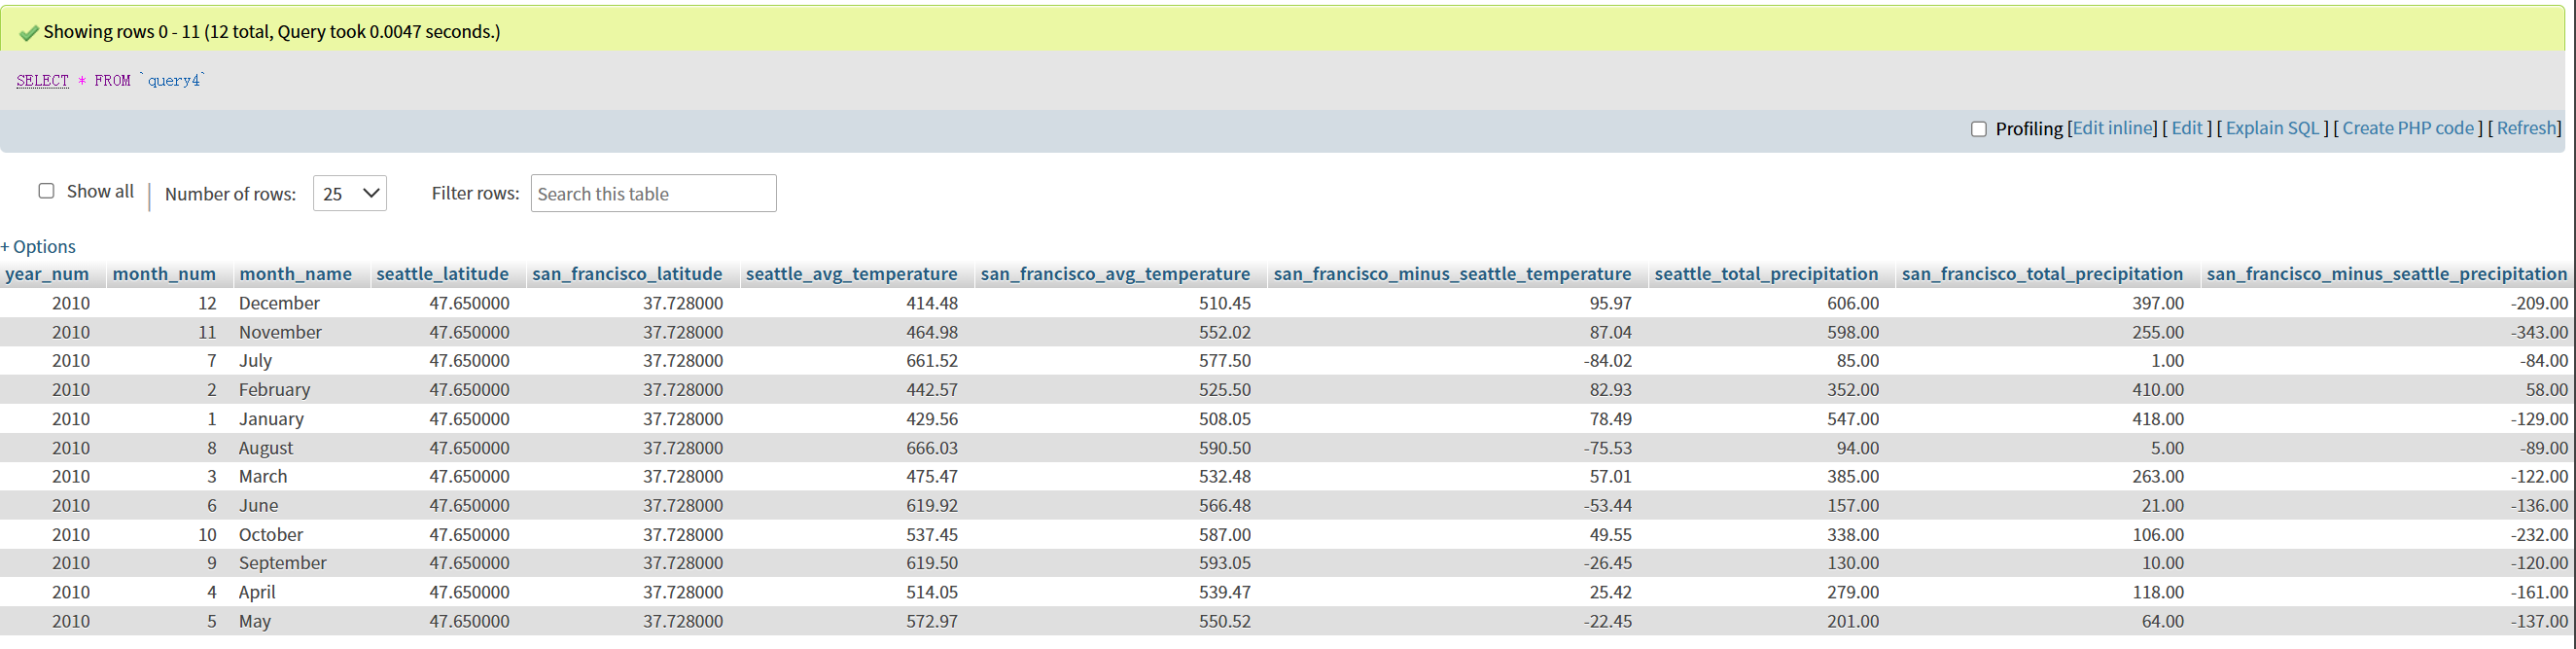
\includegraphics[width=0.95\textwidth]{OLAP_Results/query4.png}
\caption{Result of Query 4: Seattle versus San Francisco monthly difference ranking.}
\end{figure}

Query 4 compares Seattle and San Francisco month by month and ranks the months by the absolute temperature difference between the two stations. It also includes the latitude of each station and the precipitation difference for the same month. The query now computes both stations inside a single monthly comparison CTE and then ranks the resulting rows with a window function. The result is useful because it identifies the months when the climate gap between the two West Coast stations is strongest, helping connect station location with observed seasonal differences.

\subsection{Query 5: Annual Climate Profile and Wettest Month by Station}
\begin{lstlisting}[language=SQL]
-- OLAP Query 5:
-- Annual climate profile by station.
WITH annual_profile AS (
    SELECT
        station_id,
        station_name,
        year_num,
        ROUND(AVG(monthly_avg_temperature_f), 2) AS annual_avg_temperature,
        ROUND(MAX(monthly_max_temperature_f), 2) AS annual_max_temperature,
        ROUND(MIN(monthly_min_temperature_f), 2) AS annual_min_temperature,
        ROUND(
            MAX(monthly_max_temperature_f) - MIN(monthly_min_temperature_f),
            2
        ) AS annual_temperature_range,
        ROUND(SUM(monthly_total_precipitation_in), 2)
            AS annual_total_precipitation
    FROM vw_monthly_climate_imperial
    GROUP BY
        station_id,
        station_name,
        year_num
),
wettest_month AS (
    SELECT
        station_id,
        year_num,
        month_name AS wettest_month_name,
        monthly_total_precipitation_in AS wettest_month_precipitation,
        ROW_NUMBER() OVER (
            PARTITION BY station_id, year_num
            ORDER BY monthly_total_precipitation_in DESC, month_num
        ) AS precipitation_rank
    FROM vw_monthly_climate_imperial
)
SELECT
    ap.station_id,
    ap.station_name,
    ap.year_num,
    ap.annual_avg_temperature,
    ap.annual_max_temperature,
    ap.annual_min_temperature,
    ap.annual_temperature_range,
    ap.annual_total_precipitation,
    wm.wettest_month_name,
    wm.wettest_month_precipitation,
    RANK() OVER (
        PARTITION BY ap.year_num
        ORDER BY ap.annual_temperature_range DESC
    ) AS annual_temperature_range_rank
FROM annual_profile ap
JOIN wettest_month wm
    ON ap.station_id = wm.station_id
    AND ap.year_num = wm.year_num
WHERE wm.precipitation_rank = 1
ORDER BY
    ap.year_num,
    annual_temperature_range_rank,
    ap.station_name;
\end{lstlisting}

\begin{figure}[htbp]
\centering
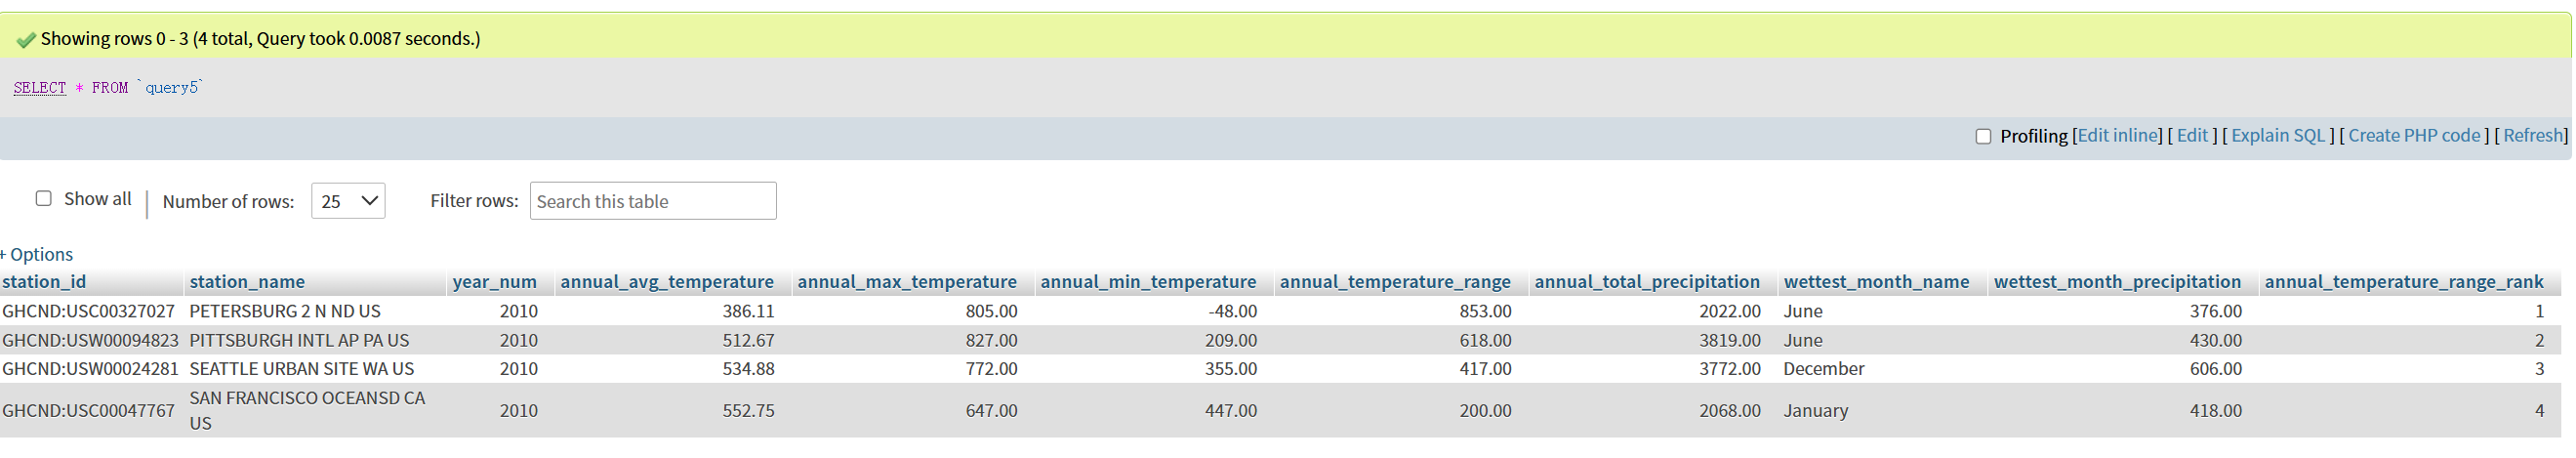
\includegraphics[width=0.95\textwidth]{OLAP_Results/query5.png}
\caption{Result of Query 5: annual climate profile and wettest month by station.}
\end{figure}

Query 5 builds an annual climate profile for each station from the shared monthly view. It calculates annual average, maximum, and minimum temperature normals, annual temperature range, annual total precipitation, and the wettest month for each station. The result supports annual-level comparison by showing which stations have the largest temperature variability and how precipitation patterns differ across locations.

\end{document}
